\chapter{Differentiation }
Derivative of $f$ at $a\in \bbR$ is $$f'(a)=\lim_{h\to 0} \frac{f(a+h)-f(a)}{h}$$To take this limit $f$ should be defined in some $(a-\eps,a+\eps)$ i.e. $f:\text{ neighborhood of }a\to\bbR$\parinf

\textbf{Goal:} Definition of $f'(a)$ for $a\in $(Some open $U$ in $\bbR^m$)$\xrightarrow{f}\bbR^n$, $a,h\in\bbR^m$\parinn

$f(a+h)-f(a)$ makes sense in $\bbR^n$ but can't divide by $h$, which is a vector in $\bbR^m$. If $m=1$ can use the same definition. ${f:\text{ Open }U\text{ in a }\bbR\to\bbR^n}$ which maps $a\mapsto(f_1(a),f_2(a),\cdots,f_n(a))$. If $n=1$ i.e. $\bbR^m\supset U\xrightarrow{f}\bbR$  we have partial derivatives.
\ex{Derivative of $f:\bbR^m\to\bbR$}{$f(x,y,z)=x^4\sin (yz)$. Here\begin{align*}
		\del{f}{x}&=4x^3\sin(yz)\\
		&=\lim_{h\to 0}\frac{f(x+h,y,z)-f(x,y,z)}{h}
\end{align*}Hence 	\begin{align*}
\left.\del{f}{x}\right|_{p=(r,s,t)}	& =\lim_{h\to 0}\frac{f(r+h,s,t)-f(r,s,t)}{h}\\
&=\lim_{h\to 0}\frac{f(p+he_1)-f(p)}{h}\qquad[p=re_1+se_2+te_3\text{ using standard basis }e_1,e_2,e_3] 
\end{align*} Its a real number if the limit exists
}
\section{Partial Derivatives:-}
\dfn{Partial Derivative  of $\bs{f:\bbR^n\supset U\to \bbR}$}{For $f: $(Open $U$ in $\bbR^m$)$\to\bbR^n$, define ``$i-$th partial derivative of $f$ at $a\in U$" to be $\left(\text{Notation }\left.\del{f}{x_i}\right|_a,\right.$ $\left.\del{f}{x_i}(a),D_if(a)\right)$ $\lim\limits_{h\to a}\frac{f(a+he_i)-f(a)}{h}\qquad(i=1,2,\cdots,m)$}

Note that this limit (if exists) is in $\bbR^n$. $$\begin{rcases*}
	\text{If }f=(f_1,f_2,\cdots,f_n)\ (f_i\text{ real}\\ \text{values in function }U\to\bbR)
\end{rcases*}\del{f}{x_i}(a)=\left(\del{f_1}{x_i}(a),\del{f_2}{x_i}(a),\cdots,\del{f_n}{x_i}(a)\right)$$So for $f:U\to \bbR^m$, $a\in U$ we get $\del{f_j}{x_i}$ where $1\leq j\leq n$ and $1\leq i\leq m$. We can arrange these  in a  matrix  of dimensions $n\times m$ $$\begin{bmatrix}
\deld{f_1}{x_1}(a) & \cdots & \deld{f_1}{x_m}(a)\\
\vdots & \ddots & \vdots\\
\deld{f_n}{x_1}(a) & \cdots & \deld{f_n}{x_m}(a)
\end{bmatrix}$$\nt{$f'(a)$ can be defined as a linear map $\bbR^n\to\bbR^m$

In the old situation $f:\bbR\to\bbR$, $f'(a)\in\bbR$ is a $1\times 1$ matrix, as such it encodes a linear map $\underset{x\mapsto f'(a)x}{\bbR\to\bbR}$
\begin{center}
	\begin{tikzpicture}
		\draw[scale=0.5,domain=-2:2, smooth, variable=\x] plot ({\x}, {\x*\x});
		\draw (0,0) node[xshift=-1.5cm,yshift=1cm]{$y=x^2$};
		\draw[scale=0.5,red,fill=red] (1,1) circle (2pt);
		\draw[scale=0.5,red] (2.5,4) node[xshift=3mm,yshift=-1cm,color=black]{slope to} -- (0,-1);
		\draw[scale=0.5] (1,1) node[xshift=6mm]{(1,1)};
		\draw[scale=0.5] (2.5,4) node[xshift=7cm,yshift=-1cm,text width=8cm]{The tangent line can be though of as the graph of linear map $\underset{t\mapsto 10t}{\bbR\to\bbR}$};
	\end{tikzpicture}
\end{center}
}
\section{Differentiation:-}
$f'(a)$ is a number such that $\lim\limits_{h\to 0}\frac{f(a+h)-f(a)-f'(a)h}{h}=0$. Inspired by this for $a\in U (\text{Open in }\bbR^m)\xrightarrow{f}\bbR^n$, we define $f'(a)$ is a linear map $\bbR^m\to\bbR^n$ such that $$\lim\limits_{h\to 0}\frac{\|f(a+h)-f(a)-f'(a)h\|}{\|h\|}=0\text{ in }\bbR $$($h$ is a small vector $\in\bbR$)
\dfn{Differentiation of $\bs{f:\bbR^m\supset U\to \bbR^n}$}{$U$ open set in $\bbR^m$, $f:U\to\bbR^n$, $a\in U$ given. We say that $f$ is differentiable  at $a$  if there is a  linear map  $T:\bbR^m\to\bbR^n$ such that $$\lim_{h\to 0}\frac{\|f(a+h)-f(a)-T(h)\|}{\|h\|}=0$$i.e $\forall\ \eps>0$, $\exists\ \delta>0$ s.t. $$\|h\|<\delta\implies \dfrac{\|f(a+h)-f(a)-T(h)\|}{\|h\|}<\eps$$We call such a linear map $T$ the derivative  of $f$ at $a$, denoted by $f'(a),D(f(a))$}
Note that $f'(a)h$ = Value of linear map $f'(a)$ applied to a vector $h$
\nt{If the above limit is 0 w.r.t any norm on $\bbR^M$ (respectively $\bbR^n$) then the same limit is 0 w.r.t any other norm on $\bbR^m$ (respectively $\bbR^n$) because \hyperref[th:all norms equiv]{all norms are equivalent}}
\begin{Theorem}{}{}
	Derivative is unique i.e. if $a\in U (\text{Open in }\bbR^m)\xrightarrow{f}\bbR^n$, and $$\lim_{h\to 0}\frac{\|f(a+h)-f(a)-T(h)\|}{\|h\|}=0 =\lim_{h\to 0}\frac{\|f(a+h)-f(a)-S(h)\|}{\|h\|}$$then $T=S$ i.e $T(v)=S(v)$ $\forall\ v\in\bbR^m$
\end{Theorem}
\begin{myproof}
	Let $R=S-T$. Want to show $R(v)=0$ $\forall \ v\in\bbR^m$ \begin{multline*}
		\frac{\|R(h)\|}{\|h\|}=\frac{\|S(h)-T(h)\|}{\|h\|}=\frac{\|(f(a+h)-f(a)-T(h))-(f(a+h)-f(a)-S(h))}{\|h\|} \\ 
		\leq \frac{\|(f(a+h)-f(a)-T(h))\|}{\|h\|}+\frac{\|(f(a+h)-f(a)-S(h))\|}{\|h\|}
	\end{multline*}Taking $\lim\limits_{h\to 0}$, we get $\lim\limits_{h\to 0}\frac{\|R(h))\|}{\|h\|}=0$.

Fix any nonzero $v$, $\lim\limits_{\lm\to 0}\lm v=0$. Take $h=\lm v$ ($\lm\neq 0$)$$\frac{\|R(h)\|}{\|h\|}=\frac{|\lm|\|R(v)\|}{|\lm|\|v\|}=\frac{\|R(v)\|}{\|v\|}$$Hence $$0=\lim\limits_{h\to 0}\frac{\|R(h)\|}{\|h\|}=\lim_{h\to 0}\frac{\|R(v)\|}{\|v\|}\implies\|R(v)\|=0\implies Rv=0$$
\end{myproof}
\qs{}{If $f:\underset{v\mapsto Av}{\bbR^m\to\bbR^n}$ is a linear map then what is $f':\bbR^m\to\bbR^n$}
\sol{See that $f'(a)=f$. (Immediate from definition)}
\qs{}{For an affine map $\underset{v\mapsto Av+c}{\bbR^m\xrightarrow{g}\bbR^n}$ for some $c\in\bbR^n$. Calculate $g'(a)$.}
\sol{$g'(a)=$ the map $h\mapsto Ah$}
\begin{Theorem}{Matrix of $f'(a)$}{}
	Prove that the matrix  of $f'(a)$ w.r.t standard basis of $\bbR^m$ and $\bbR^n$ is the Jacobian Matrix
\end{Theorem}
\begin{myproof}
	$j$th column of matrix of $T=T(e_j)\in\bbR^n$
\begin{align*}
	& \lim_{\lm\to0}\frac{\|f(a+\lm e_j)-f(a)-T(\lm e_j)\|}{\|\lm e_j\|}\text{ by definition of }T=f'(a)\\
	= & \lim_{\lm\to0}\frac{\|f(a+\lm e_j)-f(a)-\lm T(e_j)\|}{|\lm|}\begin{cases*}
		T(\lm e_j)=\lm T(e_j)\text{ by linearity} \\
		\|\lm e_j\|=|\lm|\|e_j\|=|\lm|
	\end{cases*}\\
	= & \lim_{\lm\to0}\left\|\frac{f(a+\lm e_j)-f(a)}{|\lm|}-\frac{\lm T(e_j)}{|\lm|}\right\|
\end{align*}Hence for $\lm>0$ $$\lim_{\lm\to0}\frac{f(a+\lm e_j)-f(a)}{|\lm|}-T(e_j)=0$$Let $f=\begin{bmatrix}
f_1\\ f_2 \\ \vdots\\ f_n\end{bmatrix}$. Hence \begin{align*}
T(e_j) & =\lim_{\lm\to 0}\frac{f(a+\lm e_j)-f(a)}{\lm}\\
& =\lim_{\lm\to 0}\frac{\begin{bmatrix}
	f_1(a+\lm e_j) \\
	f_2(a+\lm e_j) \\
	\vdots         \\
	f_n(a+\lm e_j)
\end{bmatrix}-\begin{bmatrix}
	f_1(a) \\
	f_2(a) \\
	\vdots \\
	f_n(a)
\end{bmatrix}}{\lm} =\begin{bmatrix}
		\deld{f_1}{x_j}(a) \\[5mm]
		\deld{f_2}{x_j}(a) \\[3mm]
		\vdots            \\
		\deld{f_n}{x_j}(a)
	\end{bmatrix}
\end{align*}Matrix of $f'(a)$= Jacobian Matrix $$\begin{bmatrix}
\deld{f_1}{x_1}(a) & \cdots & \deld{f_1}{x_m}(a)\\
\vdots & \ddots & \vdots\\
\deld{f_n}{x_1}(a) & \cdots & \deld{f_n}{x_m}(a)
\end{bmatrix}$$We have proved if $f'(a)$ exists, then  all partial derivatives  $\del{f_i}{x_j}$ exists at $x=a$ and make up the matrix  of $f'(a)$
\end{myproof}
If all $\del{f_i}{x_j}$ exists at $x=a$, does not imply  $f$ is differentiable at $x=a$?
\qs{}{Under Which conditions if all $\del{f_i}{x_j}$ exists at $x=a$, it implies that $f$ is differentiable at $x=a$?}
\begin{Theorem}{}{}
	If $f'(a)$ exists then $f$ is continuous at $x=a$
\end{Theorem}
\begin{myproof}
	If $f'(a)$ exists then $f$ is continuous at $x=a\iff\lim\limits_{h\to 0}f(a+h)=f(a)\iff\lim\limits_{h\to 0}\|f(a+h)-f(a)\|=0$
	$$\|f(a+h)-f(a)+T(h)-T(h)\|\leq \|f(a+h)-f(a)-T(h)\|+\|T(h)\|$$Now $\lim\limits_{h\to 0}\dfrac{\|f(a+h)-f(a)-T(h)\|}{\|h\|}\|h\|=0\cdot 0=0$ and $$\lim_{h\to 0}\|T(h)\|=0\text{ because }\begin{cases*}
		T\text{ is continuous (being linear) so}\\
		T(h)\to T(0)=0
	\end{cases*}$$
\end{myproof}

\section{Operator Name:-}

\section{Chain Rule:-}

\begin{Theorem}{}{}
	$\bbR^m\supset \underset{  \substack{{\uin} \\ {a}}  }{U} \underset{  \substack{\quad \\[0.25cm]\longmapsto}}{\xrightarrow{f}}   \underset{\substack{  \uin \\ b}}{  \overset{\substack{{\bbR^n} \\ \usubset}}{V}  }\xrightarrow{g}\bbR^k $. $f$ is differentiable at $a$. and $g$  is differentiable at $b=f(a)$. Then $g\circ f$ is differentiable at $a$  and $$(g\circ f)'(a)=\underbrace{g'(f(a))f'(a)}_{\substack{\text{Multiplication}\\ \text{of matrices}}}$$
\end{Theorem}
\begin{myproof}
	\subsubsection{1-Variable Case}
	$\frac{dz}{dx}=\frac{dz}{dy}\, \frac{dy}{dx}$\begin{align*}
		\frac{dz}{dx} =\lim_{\Delta x\to 0} \frac{\Delta z}{\Delta x} &=\lim_{\Delta x\to 0}\frac{\Delta z}{\Delta y}\, \frac{\Delta y}{\Delta x}\\
		& =\lim_{\Delta x\to 0}\frac{\Delta z}{\Delta y}\lim_{\Delta x\to 0} \frac{\Delta y}{\Delta x}\\
		& =\lim_{\Delta y\to 0}\frac{\Delta z}{\Delta y}\lim_{\Delta x\to 0} \frac{\Delta y}{\Delta x}\qquad [\text{As }\Delta x\to0,\ \Delta y\to 0]
	\end{align*}
\end{myproof}